\documentclass[crop,tikz]{standalone}
\usetikzlibrary{backgrounds}
\colorlet{blue}{cyan}
\tikzset{
  inverted/.style = {
    color=white,
    background rectangle/.style={fill},
    show background rectangle
  }
}
\usepackage{pgfplots}
\pgfplotsset{compat=1.13}

% Lines of constant potential for two half cylinders of radius 1 at
% position (x,y) = (0,0). The upper cylinder has constant potential V
% != 0, while the lower cylinder has constant potential V = 0.
%
% See also Jackson problem 2.13 for V_1 = V and V_2 = 0.
%
% We take the potential to be
% Phi[z_, b_:1, V_:1] := V/Pi Im[Log[-I(z + b)/(z - b)]]
%
% Inspired by the discussion in
% https://galileoandeinstein.phys.virginia.edu/Elec_Mag/2022_Lectures/EM_16_Conformal_Mapping.html

\colorlet{green}{green}

\pgfplotsset{
  inverted/.style = {
    every axis legend/.append style={
      draw=white,
      fill=black,
      text=white
    }
  }
}

\begin{document}

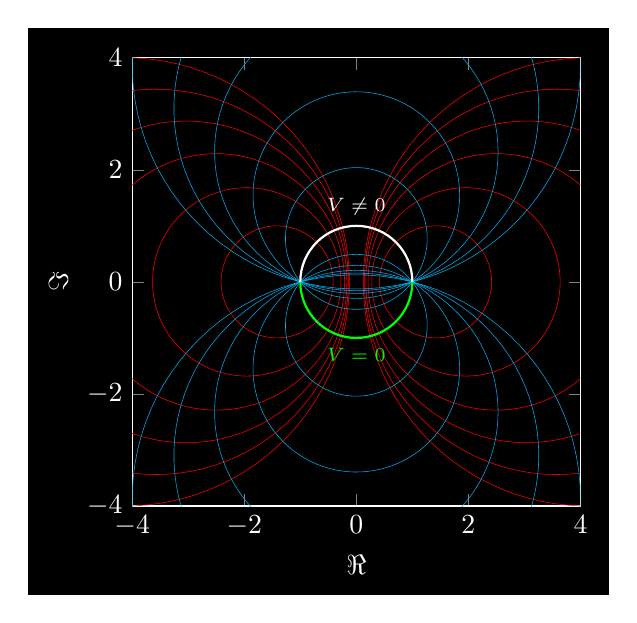
\begin{tikzpicture}[inverted,inverted]
  \pgfmathsetmacro{\numberofpotentiallines}{5};
  \pgfmathsetmacro{\numberoffieldlines}{5};
  \pgfmathsetmacro{\rmin}{1}; % minimum radius
  \pgfmathsetmacro{\rmax}{4}; % maximum radius
  \pgfmathsetmacro{\remin}{-4};
  \pgfmathsetmacro{\remax}{-\remin};
  \pgfmathsetmacro{\immin}{-4};
  \pgfmathsetmacro{\immax}{-\immin};
  \begin{axis}[inverted,
    axis equal image,
    xmin={\remin}, xmax={\remax},
    ymin={\immin}, ymax={\immax},
    xlabel={$\Re$},
    ylabel={$\Im$},
    samples=100,
    domain=0:360,
    declare function = {
      % field lines, defined by (x - c)^2 + y^2 = c^2 - 1, c^2 >= 1
      Er(\c) = sqrt(\c^2 - 1); % radius
      Ex(\x,\c) = Er(\c)*cos(\x) + \c; % x coordinate
      Ey(\x,\c) = Er(\c)*sin(\x); % y coordinate
      pc(\n,\nmax) = sqrt(\rmin^2 + 1) + \n/\nmax*(sqrt(\rmax^2 + 1) - sqrt(\rmin^2 + 1)); % calculates c
      % lines of constant potential, defined by x^2 + (y - c)^2 = c^2 + 1, for all c
      phir(\c) = sqrt(1 + \c^2); % radius
      phix(\x,\c) = phir(\c)*cos(\x); % x coordinate
      phiy(\x,\c) = phir(\c)*sin(\x) + \c; % y coordinate
      fc(\n,\nmax) = sqrt(\rmin^2 - 1) + \n/\nmax*(sqrt(\rmax^2 - 1) - sqrt(\rmin^2 - 1)); % calculates c
    },
    ]
    % field lines
    \pgfplotsinvokeforeach{0,...,{\numberoffieldlines}}{
      \addplot[red,very thin] (
      {Ex(x, pc(#1,\numberoffieldlines))},
      {Ey(x, pc(#1,\numberoffieldlines))}
      );
      \addplot[red,very thin] (
      {Ex(x, -pc(#1,\numberoffieldlines))},
      {Ey(x, -pc(#1,\numberoffieldlines))}
      );
    }
    % lines of constant potential
    \pgfplotsinvokeforeach{0,...,{\numberofpotentiallines}}{
      \addplot[blue,very thin] (
      {phix(x, fc(#1,\numberofpotentiallines))},
      {phiy(x, fc(#1,\numberofpotentiallines))}
      );
      \addplot[blue,very thin] (
      {phix(x, -fc(#1,\numberofpotentiallines))},
      {phiy(x, -fc(#1,\numberofpotentiallines))}
      );
    }
    % upper half (potential V1 != 0)
    \draw[thick] (1,0) arc (0:180:1) node[above,midway] {\scriptsize $V\neq 0$};
    % lower half (potential V2 = 0)
    \draw[thick,green] (-1,0) arc (180:360:1) node[below,midway] {\scriptsize $V=0$};
  \end{axis}
\end{tikzpicture}
\end{document}
